\documentclass[11pt]{article}
\usepackage[margin=1in]{geometry}          
\usepackage{graphicx}
\usepackage{amsthm, amsmath, amssymb}
\usepackage{setspace}\onehalfspacing
\usepackage[loose,nice]{units} %replace "nice" by "ugly" for units in upright fractions
\usepackage{graphicx}
\usepackage{color}
\usepackage{hyperref}

\usepackage{xcolor}
\definecolor{ltgrey}{HTML}{F5F5F5}


\hypersetup{
	colorlinks=true,
	linkcolor=blue,
	filecolor=magenta,      
	urlcolor=cyan,
}

\urlstyle{same}



% Use “\cite{NEEDED}” to get Wikipedia-style “citation needed” in document
%\usepackage{ifthen}
%\let\oldcite=\cite
%\renewcommand{\cite}[2]{\ifthenelse{\equal{#2}{NEEDED}}{\textcolor{red}{\ensuremath{^\texttt{[citation~needed]}}}}{\oldcite{#1}{#2}}}

\newcommand{\citationneeded}{\textsuperscript{\color{red} [citation needed]}}
 
 
\title{E-learning performance optimization with emotionally-aware visual interface}
% Viability of an emotionally-aware interface within e-learning to optimize performance
\author{Oleg Bystrov, Humboldt Universitaet zu Berlin}
\date{2018}
 
\begin{document}
\maketitle

\tableofcontents




\pagebreak

\section{Background and motivation}

E-learning providers are looking to improve the learning experience of their users and make progress as effective as possible. 
During a usual learning session each learner is subject to a range of volatile emotional states that help or hinder their learning success. 
A range of factors and stimuli, both internal and external, can influence emotions. 
When we take this knowledge about emotions into account a new way to manage a learning session opens. We can incorporate this knowledge into learning sessions and provide a more appropriate task and/or interface for the learner.

The goal of the paper is to examine a relation between emotional aspect of a user interface in an e-learning system and its effect on performance of the learner.


\begin{center}
	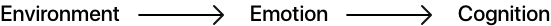
\includegraphics[width=200px]{images/relation1.png}
\end{center}
 
There is strong evidence of the surrounding environment having an influence on emotion \cite{Johnson2000, Arockiam2013, Bertamini2013}. This includes, for example, an e-learning system on the screen in front of the learner. In a similar fashion several studies have shown correlation between emotion and cognition.

\begin{center}
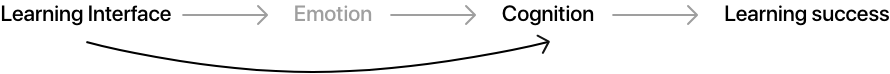
\includegraphics[width=300px]{images/relation2.png}
\end{center}

There is a logical argument of the existence of a transitive relation between these parameters, which could confirm the dependency of the edge variables. 
I.e. exposure to several interfaces each with a different emotional charge during an on-line lesson should lead to a difference in performance when working on the same task.
Insufficient research confirming this connection and explaining the effects has been published yet. 

In this paper I would like to explore to which extent the final parameter "learning success" can be influenced with the limited surface of contact that can be addressed through a learning interface on the screen.

Ethical, legal and social considerations are also part of my thesis.

\section{Approach and methods}

I propose a study that challenges human short-term memory, attention and creativity in a set of tasks. I will create a hypothetical learning environment that presents one set of activities in 2 different interfaces, intending to evoke different emotions from the user. In a blind study each subject will be assigned one of the interfaces and complete provided tasks (further described below).

Two fundamental questions to be answered:

\noindent
\colorbox{ltgrey}{
	\parbox{\textwidth}{
		\begin{itemize}
			\item Have these 2 interfaces achieved the expected emotional response?
			\item Did the results of the task vary between interfaces, as expected in accordance to the emotional response
			% sind die Ergebnisse der aufgaben unterschiedlich ausgefallen, wie erwartet in Abhängigkeit von der emotionalen Reaktion.
		\end{itemize}
	}
}

\subsection{Study design}

\begin{figure}
	\centering
	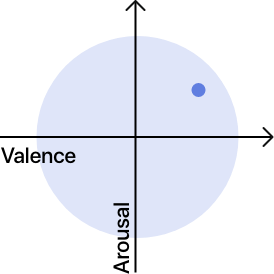
\includegraphics[width=0.25\linewidth]{images/valence-arousal.png}
	\caption[Emotions in 2 dimensions]{Emotions in 2 dimensions}
	\label{fig:valence-arousal}
\end{figure}

A usual way to represent an emotional state is through 2 attributes: arousal and valence. Arousal can range from 0 (low) to 1 (high) and valence from -1 (negative) to 1 (positive) (See figure \ref{fig:valence-arousal}). 

\textbf{1. Preconditioning:} Each test user is preconditioned to be in one of 4 states:
 \textbf{1}: Positive valence / high arousal; 
 \textbf{2}: Negative valence / high arousal;
 \textbf{3}: Positive valence / low arousal;
 \textbf{4}: Negative valence / low arousal;

One of effective sets of emotional materials is provided by the IAPS - International Affective Picture System. The system has been in developement since 1997 \cite{Lang1997} It consists of a set of images, each with an assigned arousal and valence values. With the help these materials it is possible to cause an emotional reaction from the test subject.

\begin{figure}
	\begin{center}
		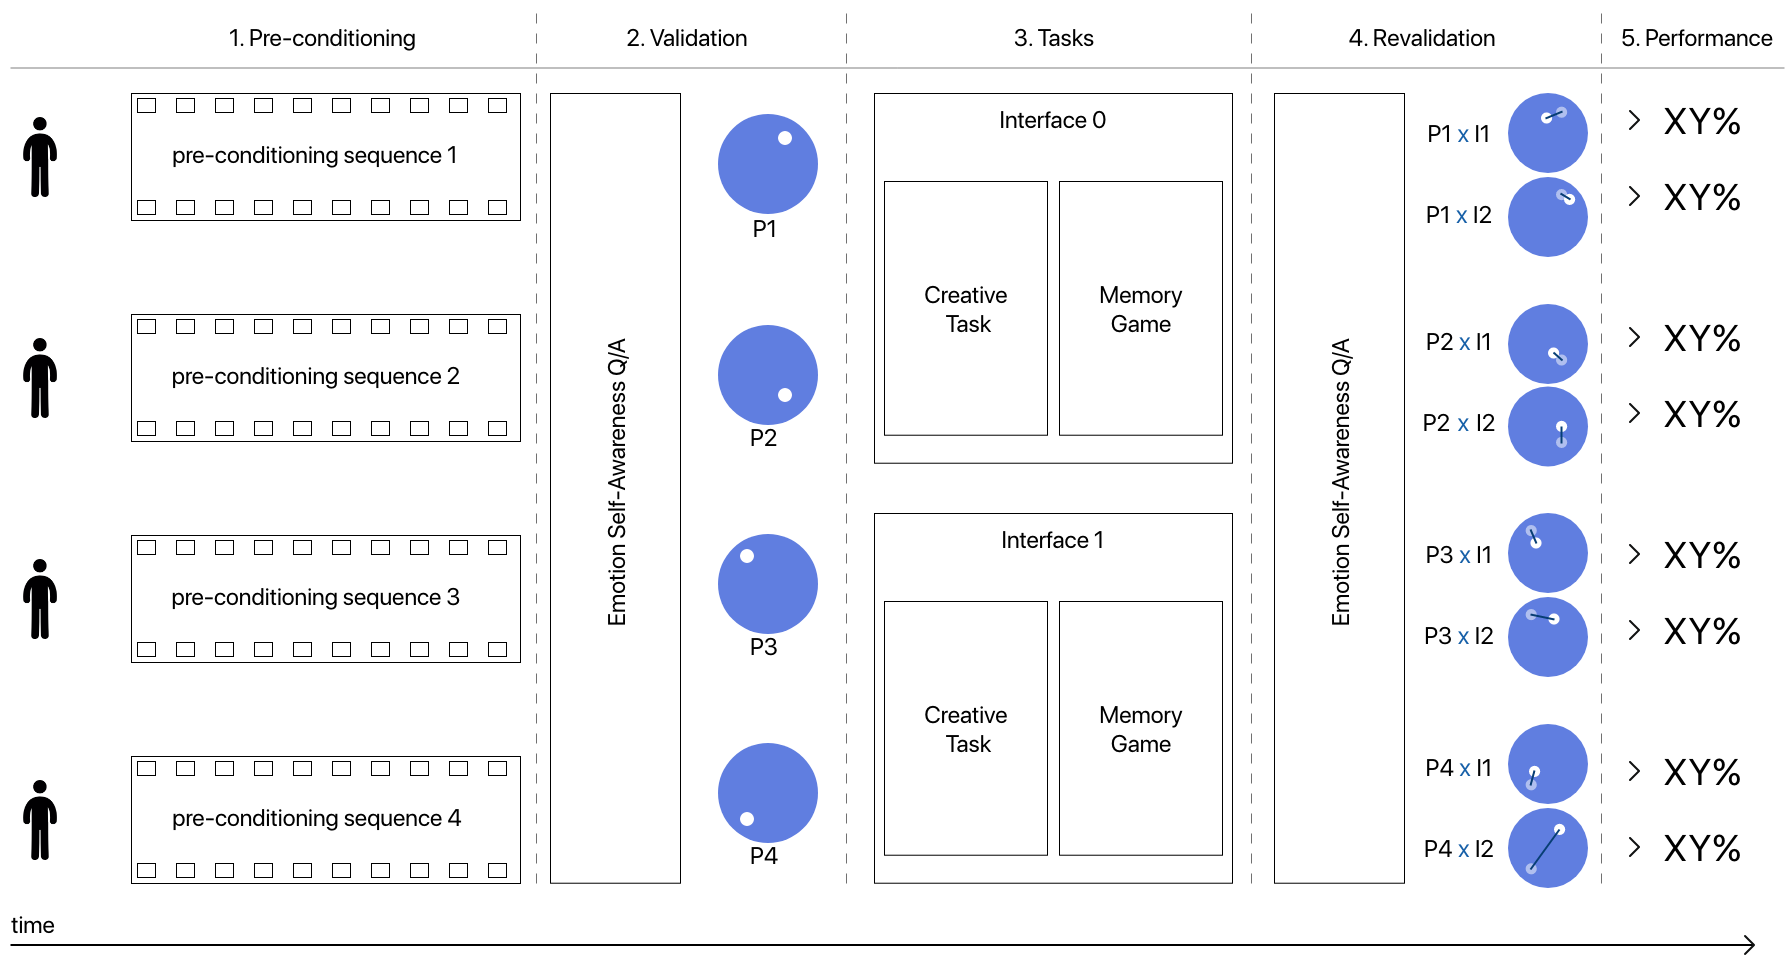
\includegraphics[width=1\textwidth]{images/study_design5.png}
		\caption{Study design\label{fig:scaled_diss}}
	\end{center}
\end{figure}

\textbf{2. Validation:} A short emotional self-awareness questionnaire will be used to validate, whether preconditioning has had sufficient and expected effect on the subject.

\textbf{3. Tasks:} A prepared task sequence (\ref{task_sequence}) will focus on testing short-term memory and creative/analytical problems. 
50\% of each group are presented with a task-set through Interface0 and 50\% would complete the tasks through Interface1.

\begin{itemize}
	\item \textbf{Interface 0 (I0):} Default interface with low emotional capacity
	\item \textbf{Interface 1 (I1):} Optimized interface with elements tailored for high arousal and positive valence (potentially optimal for both memory and analytical tasks) \cite[pp. 81 ff]{Brave2002} \cite{Heidig2015}
\end{itemize}

Both interface versions would provide equal usability features. 
The difference is in the emotional charge which stems from \underline{language used} \cite{Citron2014}, \underline{forms and shapes} \cite{Larson2012, Bertamini2013, Plass2014, Lu2012}, \underline{colors} \cite{Valdez1994, Tekirdag2015, Ou2004} \cite[p.84]{Brave2002}, and \underline{alignment} \cite{Bertamini2013} and potentially an emotional image.

\textbf{4. Revalidation:} After completing all tasks the subject will repeatedly fill out the questionnaire from step 2 to capture any changes to their emotion, caused by the interface and task. The resulting value is a vector representation of previous state and current state.
\vspace{4mm} %5mm vertical space

Effectively the study will divide subjects into 8 groups. 
It is my goal to have each testing sequence completed within about 20 minutes time to keep the subjects' time investment low.

\subsection{Measuring performance} \label{measuring}

During each task several parameters will be recorded for each subject to create a comprehensive task performance metric. 
Examples include: rate of clicks per minute, mouse movements, rate of correct answers and time elapsed until completion. 
Mouse movement and video recordings could allow further qualitative analysis and provide room for more insight.

\subsection{Task Sequence} \label{task_sequence}

Psychological and cognitive studies have developed a variety of tests evaluating abilities of human mind. 
They differ in the art of activity and their focus, for example some concentrate on memory, creative thinking, analytical thinking, solving mathematical problems, imagination or orientation capabilities.

For this study I found several potentially fitting tests:

- \textbf{a classic memory game}. The goal is to find all pairs of images on a raster of (ex. 10 by 10) tiles. 
Only 2 pieces can be turned over at once. 
After which they turn back around and another try of finding a pair starts. 
In the context of this study several adjustments will reduce the ratio of luck/chance involved in choosing correct tiles: Showing all cards at the beginning, discarding the correct tile choices at the end of the game when few tiles left unturned, and others.

- \textbf{Remote Associates Test}. Originally published in 1962 by \cite[p.226 ff]{Mednick1962}, this test evaluates individual creativity. 
The test subject is presented with a set of 3 words and they must find a fourth word that is in some way connected to all three words.

\subsection{Evaluation}

Usually a quantitative analysis can yield better results with a larger number of subjects.
I expect to attain a minimum of 15 subjects per group (15 * 8 = 120 ). But the more I can get - the better.
To simplify acquisition of test subjects I will create a testing environment in the form of a web-application (explained section \ref{implementation}) and spread it through online media to be completed remotely.
Additional steps within the application will be taken to minimize risk of noise and false results that come from this type of testing. Part of the study will be conducted in a controlled environment on university grounds.

\section{Implementation} \label{implementation}

To facilitate the study I will build a web-application (based on reactjs), runnable on desktop and tablet devices. Data emitted from the application will be saved in a remote database (mongodb) for the purposes of evaluation.

Some open source software might be used and integrated into the system when applicable. E-learning tasks development is not an integral part of this thesis, although potential technological basis for integration of emotion information in e-learning systems will be discussed.

No information should be stored locally on the device after finishing a session.

\section{Implications of the study}

If this study can demonstrate a significant difference in performance across groups, we can conclude that emotional features of digital user interface can have a noticeable impact on the way people consume information, memorize and analyze problems.
It will pave the way for further studies being done exactly which aspects of an interface have the biggest impact and how to design for sustained attention and performance.

E-learning providers can use these findings to better structure their online lessons and invest in design that supports the learner.

Further these findings can be adapted and generalized to make use of within other applications in software, digital media and similar outlets.



\clearpage

% \section {Problem description}

E-Learning systems provide a convenient, scalable way to convey and share knowledge. They allow a student to learn material at their own preferred pace. 
Current state of-the-art e-learning systems furthermore include a training component with intelligent tailored guidance for completion. 

Such systems come close to an actual learning environment in a school, but are limited due to their technology and remote nature. More precisely, these systems lack an “emotional” component that can be expressed in a more personal setting. Devices like eye-movement trackers, pulse-, and various other vital-sign-trackers can be introduced to improve on this limitation. Such additional information can create an environment where a better and more intelligent personal one-on-one guidance system becomes a possibility.

Learning performance analysis is an ever-present subject of educational research. Understanding how and when we learn and memorize material in the most efficient way would allow to tune learning systems and increase their effectiveness. Studies have shown that emotion is central in the cognitive process \cite{ORegan2003}, feeling can influence the learning process. \cite{Hawkins2017} 

Past research highlights the importance of the state of learners mind for a successful learning process, yet there has been insufficient research on user interfaces (which a possible with e-learning systems) and their capacity to arouse and support an emotional and cognitive state, that is beneficial for learning.

%Bisherige Forschung.
%Forschungslücke behaubten
%Lücke füllen

\section{Goals of the paper}

The paper will explore the processes of consuming knowledge in an e-learning environment, methods for extracting and understanding the emotional and cognitive state of the learner (may be not this part), as well as provide suggestions to guiding and influencing the state to achieve better learning performance with UX and UI techniques.

The first goal of the paper is to conceptually create a prototype that would propose certain actions based on possible input data in the system. Furthermore, to create a technological infrastructure for consuming data from the available sources and transforming it in a way appropriate to the target e-learning system. Third, analyse and propose different approaches to guiding a lesson with additionally available data and to build a working prototype module for the target e-learning system including visualisation of historical lesson performance and real-time lesson guidance system.

\section{Approach and methods}

The first section of the paper will focus on visual presentation of historical and real-time data to provide users of the e-learning system with best appropriate information during a lesson and after it for the purposes of analysis.

I will explore the possibilities of supported and automatic decision making by the system to best decide which content to deliver to the user. Furthermore, I will propose ways of extracting emotional state of the user with direct user input to augment sensor data provided by the tracker.

The second section will focus on technology needed to integrate and run on the system of the end-user (a web-browser) and develop a suitable api to support several requirements of the analytical system.

\section{Implementation}

There are several considerations in developing an unobtrusive and supportive extension to an e-learning platform. These include:

\begin{itemize}
	\item Technological complexity of providing near-real-time data to the system and being able to compute context-sensitive and time-relevant actions based on received input.
	\item Psychological approach that considers human traits and reactions to stimuli, making correct assumptions of the human state of mind
	\item Visual language that responds to the input in an unobtrusive and supporting way, guiding but not disturbing the learning process
\end{itemize}

\section{Scheduling}
\begin{itemize}
	\item February, March – Research and defining the structure as well as concrete goal
	\item March, April – concept development and research basis, writing
	\item End of May registration of Thesis.
	\item May, June – writing and describing concept (concept at the end of the period is done and developed)
	\item July, Aug – writing analysis, possible revisions and adjustments based on feedback and further findings (possibly user testing)
\end{itemize}


\section{Sources}

Human Computer Interaction, Alan Dix, 2003, Prentice Hall
ISBN-13: 978-0130461094

Information Dashboard Design: Displaying Data for At-A-Glance Monitoring, Stephen Few, 2013, Analytics Press
ISBN-13: 978-1938377006



\bibliographystyle{apalike}
\bibliography{Library/Masterarbeit.bib}

\end{document}